\documentclass{article}

\usepackage[french]{babel} 
\usepackage[T1]{fontenc}
\usepackage{lmodern}
\usepackage[utf8]{inputenc}

\usepackage{float}
\usepackage{mathtools}
\DeclarePairedDelimiter{\ceil}{\lceil}{\rceil}
\usepackage{fancyhdr}
\usepackage{extramarks}
\usepackage{amsmath}
\usepackage{amsthm}
\usepackage{amsfonts}
\usepackage{amssymb}
\usepackage{tikz}
\usepackage{graphicx}
\usepackage{pdfpages}
\usepackage[makeroom]{cancel}
\usepackage{karnaugh-map}

%
% Basic Document Settings
%

\topmargin=-0.45in
\evensidemargin=0in
\oddsidemargin=0in
\textwidth=6.5in
\textheight=9.0in
\headsep=0.25in

\linespread{1.1}

\pagestyle{fancy}

%
% Create Problem Sections
%

\newcommand{\enterProblemHeader}[1]{
    \nobreak\extramarks{}{Question \arabic{#1} continued on next page\ldots}\nobreak{}
    \nobreak\extramarks{Question \arabic{#1} (suite)}{Suite de la question \arabic{#1} à la page suivante\ldots}\nobreak{}
}

\newcommand{\exitProblemHeader}[1]{
    \nobreak\extramarks{Question \arabic{#1} (suite)}{Suite de la question \arabic{#1} à la page suivante\ldots}\nobreak{}
    \stepcounter{#1}
    \nobreak\extramarks{Question \arabic{#1}}{}\nobreak{}
}

\setcounter{secnumdepth}{0}
\newcounter{partCounter}
\newcounter{homeworkProblemCounter}
\setcounter{homeworkProblemCounter}{1}
\nobreak\extramarks{Question \arabic{homeworkProblemCounter}}{}\nobreak{}

%
% Homework Problem Environment
%
% This environment takes an optional argument. When given, it will adjust the
% problem counter. This is useful for when the problems given for your
% assignment aren't sequential. See the last 3 problems of this template for an
% example.
%
\newenvironment{homeworkProblem}[1][-1]{
    \ifnum#1>0
        \setcounter{homeworkProblemCounter}{#1}
    \fi
    \section{Tâche \arabic{homeworkProblemCounter}}
    \setcounter{partCounter}{1}
    \enterProblemHeader{homeworkProblemCounter}
}{
    \exitProblemHeader{homeworkProblemCounter}
}

%
% Homework Details
%   - Title
%   - Due date
%   - Class
%   - Section/Time
%   - Instructor
%   - Author
%

\newcommand{\hmwkTitle}{Travail\ pratique\ 4}
\newcommand{\hmwkDueDate}{8 Décembre 2023}
\newcommand{\hmwkClass}{\ \ IFT 3913}
\newcommand{\hmwkClassTime}{}%Section 
\newcommand{\hmwkClassInstructor}{Professeur: Michalis Famelis}
\newcommand{\hmwkAuthorName}{\textbf{Killian Gervais \& Gabriel Hazan}}

%
% Title Page
%

\title{
    \vspace{2in}
    \textmd{\textbf{\hmwkClass:\ \hmwkTitle}}\\
    \normalsize\vspace{0.1in}\small{Pour\ le\ \hmwkDueDate\ à 23:59 }\\
    \vspace{0.1in}\large{\textit{\hmwkClassInstructor\ \hmwkClassTime}}
    \vspace{3in}
}

\author{\hmwkAuthorName}
\date{}

\renewcommand{\part}[1]{\textbf{\large Partie \Alph{partCounter}}\stepcounter{partCounter}\\}

% Probability commands: Expectation, Variance, Covariance, Bias
\newcommand{\E}{\mathrm{E}}
\newcommand{\Var}{\mathrm{Var}}
\newcommand{\Cov}{\mathrm{Cov}}
\newcommand{\Bias}{\mathrm{Bias}}

\tikzstyle{bag} = [align=center]
\begin{document}

\maketitle
\thispagestyle{empty}

\pagebreak
% Tache 1
\begin{homeworkProblem}
    D'après la spécification donnée, on a deux types d'entrées: les devises (\textit{currencies}) et les montants (\textit{amounts}). Soit les devises du programme $P_C$ défini sur \{USD, CAD, GBP, EUR, CHF, AUD\} avec \\$C$ = Currencies = \{USD, CAD, GBP, EUR, CHF, AUD, JPY, INR, NZD\}, cette dernière pourrait être agrandie au besoin, et les montants du programme $P_A$ défini sur [0, 1 000 000], l'intervalle des valeurs valides, avec $A$ = Amounts = Réels positifs.\\
    \linebreak
    Il y a deux classes d'équivalences pour les devises:
    \begin{itemize}
        \item[$\bullet$] Les valeurs d'entrées valides:\quad $C_1 = P_C =$ \{USD, CAD, GBP, EUR, CHF, AUD\}
        \item[$\bullet$] Les valeurs d'entrées invalides:\quad $C_2 =$ \{JPY, IRN, NZD\}
    \end{itemize}
    On choisit une valeur de chaque classe, pour pouvoir tester le cas ou l'une des devises est valide tandis que l'autre ne l'est pas, ainsi qu'une seconde valeur de devise valide pour tester les conversion de montant pour créer notre jeu de test $T_C$ = \{USD, EUR, JPY\}.\\
    \linebreak
    Pour les montants, il y a trois classes d'équivalences, $a \in \mathbb{R}$:
    \begin{itemize}
        \item[$\bullet$] Les valeurs appartenant à $P_A$:\quad $A_1 = \{0 \leq a \leq 1\ 000\ 000\}$
        \item[$\bullet$] Les valeurs invalides inférieures à $P_A$:\quad $A_2 = \{a < 0\}$
        \item[$\bullet$] Les valeurs invalides supérieure à $P_A$:\quad $A_3 = \{a > 1\ 000\ 000\}$
    \end{itemize}
    On choisit choisit une valeur "typique" dans chaque classe d'équivalence et plusieurs aux bornes de celles-ci pour créer le jeu de test $T_A = \{-2\ 222\ 222, -0.09, 0, 500\ 000, 1\ 000\ 000, 1\ 000\ 000.01, 2\ 222\ 222\}$.\\

    Si une entrée est invalide, on s'attend à ce que le code ne s'arrête pas, il est donc capable de s'adapter à une mauvaise entrée fournie par l'utilisateur, que ce soit pour une devise ou un montant. On s'attend a ce que ce soit la classe MainWindow qui gère les entrées invalides. Puisque, selon la spécifiation, le type des données retournées par ces méthodes sont des double positifs on s'attend à recevoir "-1.0" comme résulat lors d'une entrée invalide.
\end{homeworkProblem}

%Tache 2
\begin{homeworkProblem}
    On va suivre la méthode des 5 critères de sélection de jeux de tests de la méthode boîte blanche dans le but de créer nos jeux de tests, lorsque ceux-ci sont applicables.\\
    \hfill\\
    Commençons par la méthode \textit{convert} de la classe MainWindow:
    \begin{itemize}
        \item[\underline{Couverture des instructions}:]
        Puisque les boucles utilisées sont des \textit{for} il suffit que $currencies.size() > 0$ pour que les boucles soient exécutées au moins une fois, avec \textit{currencies} la liste des devises acceptées. Les structures conditionnelles sont toutes des \textit{if}, leur code est exécuté si leur condition est vraie. De plus, on note que le premier et le troisième sont dans les boucles \textit{for}. Le code du premier \textit{if} est exécuté quand \textit{currency2} est dans la liste des devises, même chose pour le code du troisième mais avec \textit{currency1} cette fois. Le code du dernier, qui est en fait le second \textit{if} de la méthode, est exécuté lorsque le code du premier l'a été, ils partagent donc la même classe du domaine. D'après cela, on obtient la classe d'équivalence suivante:\\
        $D_1$ = \{(\textit{currency1}, \textit{currency2}) | \textit{currencies.size()} > 0\ \&\ \textit{currency1}, \textit{currency2} $\in$ \textit{currencies}\}\\
        Avec celle-ci, tout le code est exécuté au moins une fois. On peut donc prendre le jeu de test: \{"US Dollar", "Euro"\}, ces deux valeurs étant définies dans la classe Currency.
        
        \pagebreak
        
        \item[\underline{Couverture des arcs du graphe de flot de contrôle}:] On obtient le graphe de flot contrôle suivant
        \begin{figure}[H]\centering
            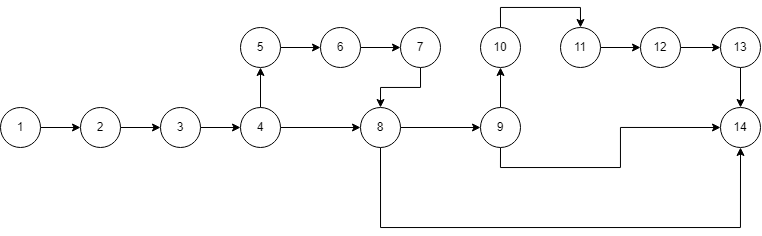
\includegraphics[width = \linewidth]{control-flow-graph-MainWindow.png}
        \end{figure}
        Les numéros correspondent à la ligne de code qui n'est pas un commentaire correspondante dans la méthode, 1 la première ligne après le bracket d'ouverture. On déjà énoncé les conditions qui font que les \textit{if} et les boucles \textit{for} sont exécutés ci-haut. On veut cependant ajouter les cas qui font que leur conditions sont fausses. D'où:\\
        $D_1$ = \{(\textit{currency1}, \textit{currency2}) | \textit{currencies.size()} > 0 \& \textit{currency1}, \textit{currency2} $\in$ \textit{currencies}\}\\
        $D_2$ = \{\textit{curr.1}, \textit{curr.2}) | \textit{currencies.size()} = 0\}\\
        $D_3$ = \{(\textit{currency1}, \textit{currency2})|\textit{currencies.size()} > 0, \textit{currency1}$\not\in$\textit{currencies} \& \textit{currency2}$\in$\textit{currencies}\}
        $D_4$ = \{(\textit{currency1}, \textit{currency2})|\textit{currencies.size()} > 0, \textit{currency1}$\in$\textit{currencies} \& \textit{currency2}$\not\in$\textit{currencies}\}\\
        \hfill\\
        Il n'y a pas le cas où les deux devises ne sont pas dans la liste, puisque si la deuxième ne l'est pas alors la partie du code qui vérifie si la première se trouve dans la liste n'est pas exécutée. On peut donc prendre le jeu de test suivant: \{\{("US Dollar", "Euro") | \textit{currencies = $\emptyset$}\}, \{("US Dollar", "Euro"), ("Australian Dollar", "US Dollar"), ("Euro", "US Dollar") | "US Dollar", "Euro" $\in$ \textit{currencies}\}\}, puisque le dollar australien n'est pas défini dans Currency tandis que les deux autres le sont.\\
        
        \item[\underline{Couverture des chemins indépendants du graphe de flot de contrôle}:] La compléxité cyclomatique est\\ $V(G) = e-n+2 = 18 - 14 + 2 = 1 + d = 1 + 5 = 6$. On définit maintenant une base de 6 chemins indépendants du graphe de flot:
        \begin{itemize}
            \item[$\bullet$] 1-2-3-4-8-14: la liste des devises est vide, $D_1$ = \{(\textit{currency1}, \textit{currency2}) | \textit{currencies = $\emptyset$}\}
            \item[$\bullet$] 1-2-3-4-5-4-8-14: $D_2$ = \{(\textit{currency1}, \textit{currency2}) | \textit{currency2} $\not\in$ \textit{currencies}, \textit{currency1} $\in$ \textit{currencies}\}
            \item[$\bullet$] 1-2-3-4-5-6-7-8-9-10-9-14: $D_3$ = \{(\textit{curr.1}, \textit{curr.2}) | \textit{curr.2} $\in$ \textit{currencies}, \textit{curr.1} $\not\in$ \textit{currencies}\}
            \item[$\bullet$] 1-2-3-4-5-6-7-8-9-10-11-12-13-14: $D_4$ = \{(\textit{curr.1}, \textit{curr.2}) | \textit{curr.2}, \textit{curr.1} $\in$ \textit{currencies}\}
        \end{itemize}
        On a utilisé tous les arcs du graphe et il ne reste donc plus de chemins linéairement indépendants. Le jeu de test créer à l'étape précédente répondait déjà à ces critères, on le conserve donc tel quel.\\

        \item[\underline{Couverture des conditions}:] Il n'y a pas de conditions composées dans cette méthode. Ce critère n'est donc pas applicable.\\
        
        \item[\underline{Couverture des i-chemins}:] Les deux boucles sont des boucles simples. Il n'y a pas un grand intêret à faire l'ensemble des cas proposées par ce critère puisque le nombre d'itération n'impact pas le résultat. Les cas intéressant sont: on saute la boucle, ce qui se fait lorsque \textit{currencies.size() = 0}, on effectue $m$ itérations, ce qui arrive lorsque les devises sont dans la liste, la valeur de m n'est pas importante du moment que $0< m < n$, et on effectue n itérations, ce qui "arrive" lorsque l'une des devises n'est pas dans la liste. Or, le jeux de test conçu répond déjà à tout cela. Notre jeu de test le plus couvrant est donc:\\ $T$ = \{\{("US Dollar", "Euro") | \textit{currencies = $\emptyset$}\}, \{("US Dollar", "Euro"), ("Australian Dollar", "US Dollar"), ("Euro", "US Dollar") | "US Dollar", "Euro" $\in$ \textit{currencies}\}\}
    \end{itemize}
    
    \pagebreak
        
    Et maintenant, la méthode \textit{convert} de la classe Currency:
    \begin{itemize}
        \item[\underline{Couverture des instructions}:] Tout ensemble de paires de nombres réels positifs va permettre à chaque instruction d'être exécutée au moins une fois. Un jeu de test valide est donc: $T = \{(1234.56, 789)\}$\\
        
        \item[\underline{Couverture des arcs du graphe de flot de contrôle}:] On obtient le graphe de flôt de controle suivant:
            \begin{figure}[H]\centering
                
\includegraphics[width = .44\linewidth]{control-flow-graph-Currency.png}
                \caption{Flot de contrôle de la méthode \textit{convert} de la classe Currency}
                \label{fig:enter-label}
            \end{figure}
        Le critère n'est pas pertient puisque l'on a une simple séquence d'instructions sans branchements de contrôles conditionnels. On peut garder le même jeu de test qu'à l'étape précédente.\\
        
        \item[\underline{Couverture des chemins indépendants du graphe de flot de contrôle}:] Ici encore, le critère est applicable mais peu pertinent puisque $V(G) = e-n+2 = 3 - 4 + 2 = 1 + d = 1 + 0 = 1$. Il y a donc un unique chemin que l'on suit déjà avec le jeu de test que l'on a définit.\\
        \item[\underline{Couverture des conditions}:] Non applicable puisqu'il n'y a pas de conditions dans cette méthode.\\
        \item[\underline{Couverture des i-chemins}:] Non applicable puisqu'il n'y a pas de boucles dans cette méthode.\\
    \end{itemize}
    
    
\end{homeworkProblem}

%Tache 3
\begin{homeworkProblem}
    On aurait du ajouter une seconde valeur de devise invalide afin de tester le cas de conversion une devise invalide vers une devise invalide
        
    Pour la methode boite noire puisque l'on ne connait pas l'implementation des methodes on a assume que c'est dans la classe MainWindow que la validation des erreurs se fait puisque l'on s'attend a ce que celle-ci utilise la classe Currency. On s'attendait donc a ce que \textit{Currency.convert} convertise toutes paires de nombres reels et c'est pourquoi on a utilise les meme valeurs numeriques que pour les tests de \textit{MainWindow.convert}, soit le jeu de test $T_A$ definit dans la tache 1, on ne se soucit pas des taux de changes puisqu'ils ne font pas partis de la specification. Les resultats des tests sont ce qui etait attendu. Pour tester \textit{MainWindow.convert} on a utilise $T_C$ et $T_A$ puisque celle-ci requiere les deux types d'entrees enonce par la specification. On a convertie la version raccourci des noms des devises a leur noms coomplets dans les tests puisque l'on a vu que l'interface utilise ces derniers. On a assume que lorsqu'un montant ou une des devises ne repondait pas a la specification la methode retourne "-1.0". Ce n'est visiblement pas le cas ce qui fait que seuls les tests dont le montant et les deux devises sont valide n'echouent pas tandis que tous les autres test echouent. N'ayant pas acces au code on ne peut dire pourquoi le resultat attendu n'est pas celui que l'on veut avec cette methode. On a teste le comportement avec l'une des devises qui est invalide tandis que l'autre l'est (nous n'avons pas donne d'importance au montant puisque le comportement attendu ne change pas en fonction de celui-ci), les deux devises sont valides et le montant l'est aussi, les deux devises sont valides mais le montant ne l'est pas.\\

    Pour la methode boite blanche on a utilise les jeux de tests que nous avons definit dans la tache 2. Pour \textit{MainWindow.convert}, tous les criteres etaient applicables sauf celui des conditions puisqu'il n'y a pas de conditions composees dans la methode. Les cas couverts par nos tests sont: onsaute les boucles, on effectue m iterations, une des devises n'est pas dans la liste des devises. Les autres cas ne sont pas plus interessants pour nous (justification dans la tache 2). Cette fois-ci tous les tests passent puisque l'on sait maintenant comment la methode fonctionne. Pour \textit{Currency.convert}, seuls le critere de couverture des instructions est vraiment pertinent, puisque la methode est tres simple. On peut tout de meme applique la plupart sauf les criteres de couverture des conditions et des i-chemins (precision dans tache 2). On obtient du critere de couverture des instructions un jeu de test tres simple qui nous permet de confirmer que la methode marche comme attendue avec notre test. On a pas besoin de plus d'un cas puisque l'on sait que cela est generalisable a l'ensemble des paires de reels positifs.\\

    La methode boite noire a l'incovenient que des tests que l'on pense bons ne le sont pas puisque l'on ne sait pas exactement comment le programme est code mais elle est rapide est facile. En comparaison, la methode boite blanche est beaucoup plus longue est complexe. Elle permet cependant d'obtenir une couverture maximale du code avec de meilleurs resultats et moins de tests a ecrire.
\end{homeworkProblem}
\end{document}